\documentclass[a4paper]{article}
\usepackage{geometry}
\geometry{a4paper,left=2.7cm,right=2.7cm,top=2.54cm,bottom=2.54cm}
 
%导入ctex包
\usepackage[UTF8,heading=true]{ctex}
 
\usepackage[utf8]{inputenc}
\usepackage[linesnumbered,ruled,vlined]{algorithm2e}
\usepackage{amsmath}
\usepackage{xcolor}
\usepackage{array}
\usepackage{subcaption}


%设置摘要格式
\usepackage{abstract}
\setlength{\abstitleskip}{0em}
\setlength{\absleftindent}{0pt}
\setlength{\absrightindent}{0pt}
\setlength{\absparsep}{0em}
\renewcommand{\abstractname}{\textbf{\zihao{4}{摘要}}}
\renewcommand{\abstracttextfont}{\zihao{-4}} %设置摘要正文字号
 
%设置页眉和页脚，只显示页脚居中页码
\usepackage{fancyhdr}
\pagestyle{plain}
 
%调用数学公式包
\usepackage{amssymb}

 
%调用浮动包
\usepackage{float}
\usepackage{subfig}
\captionsetup[figure]{labelsep=space} %去除图标题的冒号
\captionsetup[table]{labelsep=space} %去除表格标题的冒号
%设置标题格式
\ctexset{
	%设置一级标题的格式
	section = {
		name={,、},
		number=\chinese{section}, %设置中文版的标题
		aftername=,
	},
	%设置三级标题的格式
	subsubsection = {
		format += \zihao{-4} % 设置三级标题的字号
	}
}
 
 
%使得英文字体都为Time NewTown
%\usepackage{times}
 
%图片包导入
\usepackage{graphicx}
\graphicspath{{figures/}} %图片在当前目录下的figures目录
 
%参考文献包引入
\usepackage{cite}
\usepackage[numbers,sort&compress]{natbib}
 
%代码格式
\usepackage{listings}
\usepackage{graphicx}%写入python代码
\usepackage{pythonhighlight}%python代码高亮显示
\lstset{
	%numbers=left, %设置行号位置
	%	numberstyle=\tiny, %设置行号大小
	keywordstyle=\color{blue}, %设置关键字颜色
	commentstyle=\color[cmyk]{1,0,1,0}, %设置注释颜色
	escapeinside=``, %逃逸字符(1左面的键)，用于显示中文
	breaklines, %自动折行
	extendedchars=false, %解决代码跨页时，章节标题，页眉等汉字不显示的问题
	xleftmargin=1em,xrightmargin=1em, aboveskip=1em, %设置边距
	tabsize=4, %设置tab空格数
	showspaces=false %不显示空格
}
 
 
\renewcommand{\refname}{}
 
%item包
\usepackage{enumitem}
 
%表格加粗
\usepackage{booktabs}
 
%设置表格间距
\usepackage{caption}
 
%允许表格长跨页
\usepackage{longtable}
 
%伪代码用到的宏包
\usepackage{algorithmic}
\usepackage{algorithm}
 
%正文区
\title{论文标题} 
\date{} %不显示日期
 
%文档
\begin{document}
	\maketitle
	\vspace{-6em} %设置摘要与标题的间距
	\zihao{-4} %设置正文字号
	%摘要部分
	\begin{abstract}
		
		\hspace{0.2em}\textbf{针对问题一}，...
		
		\textbf{针对问题二}，...
		
		\textbf{针对问题三}，...
		
		\textbf{针对问题四}，...、、
		%关键词（上文最后一段要用“\\”换行）
		\newline
		\noindent{\textbf{关键词：} \textbf{关键词1}\quad   \textbf{关键词2}\quad \textbf{关键词3} \quad \textbf{关键词4}\quad \textbf{关键词5}} 
	\end{abstract}
	
	\clearpage %换页
	
	%正文部分
	%Part one
	\section{问题背景与重述}
	\subsection{问题背景}
 
	%\begin{figure}[H]
	%	\centering %图片居中
	%	\captionsetup{skip=4pt} % 设置标题与表格的间距为4pt
	%	\includegraphics[width=10cm]{图片文件名} %width设置图片大小
	%	\caption{商超蔬菜示意图\label{商超蔬菜示意图}} %设置图片的标题及引用标签
	%\end{figure}
	
	\subsection{问题重述}
	\begin{enumerate}[itemindent=0.5cm]
		\item ...	\item ...
		\item ...
		\item ...
	\end{enumerate}
	
	%Part Two
	\section{问题分析}
	\subsection{问题一的分析}






	\subsection{问题二的分析}
	
	
	\subsection{问题三的分析}
	\subsection{问题四的分析}
	
	%Part Three
	\section{模型假设}
	%假设的列表
	\begin{enumerate} 
		\item 
		\item 
		\item 
		\item 
	\end{enumerate}
	
	%Part Four
	\section{符号说明}
	%浮动体表格，使用table实现
	\begin{table}[H] %[h]表示在此处添加浮动体，默认为tbf，即页面顶部、底部和空白处添加
		\captionsetup{skip=4pt} % 设置标题与表格的间距为4pt
		\centering
		\setlength{\arrayrulewidth}{2pt} % 设置表格线条宽度为1pt
		\begin{tabular}{cc} %c表示居中，l表示左对齐，r表示右对齐，中间添加“|”表示竖线
			\hline
			\makebox[0.15\textwidth][c]{符号} & \makebox[0.6\textwidth][c]{说明}  \\ 
			\hline
			r & Spearman系数  \\
			 &   \\
			 &   \\
			 &   \\
			\hline
		\end{tabular}
		% \hline是横线，采用\makebox设置列宽
	\end{table}
	
	
	%Part Five
	\section{模型的建立与求解}
	\subsection{问题一：简化结构下基于基本模型的规划模型}
	\subsubsection{第一小问模型的建立与求解}

题目要求设定高压油管中燃油的期望压力为$P_e=100MPa$，设计单向阀开启时常T，使得一定时间里高压油管燃油实际压力的偏差值达到最小；假设研究的时间段为$[t_1,t_2]
$;
\\于是设决策变量为
\begin{equation}
   T
 \end{equation}
\\目标函数为
\begin{equation}
minZ=\int_{t_1}^{t_2}(P(t)-P_e)^2  \,dt 
 \end{equation}
\\约束条件有：
\\（1）模型满足基本模型的方程组(8)(9)
\\（2）模型满足燃油密度和燃油压力方的关系$P=g(\rho )$
\\即
\begin{equation}
\begin{cases}
	\frac{dm}{dt}=\rho_1\cdot I-\rho(t)\cdot E \\
P=g(\rho )\\
m(0)=\rho (0) \cdot  V
\end{cases}
\end{equation}
\\其中


\begin{equation}
\begin{cases}
\rho(t)=\frac{m(t)}{V} \\
I(t)=\begin{cases}Q_1(t),t\in \varOmega _{1,t}\\0,$其他$\end{cases},i=1,2,\ldots ,n_1\\
E=\begin{cases}Q_2(t),t\in \varOmega _{2,t}\\0,$其他$\end{cases},i=1,2,\ldots ,n_2\\
Q_1(t)=CA\sqrt{\frac{2\Delta P(t)}{\rho(t)} }\\
Q_2(t)=\begin{cases}100t',t'\in[0,0.2)\\
20,t'\in[0.2,2,2)\\
240-100t',t'\in[2.2,2.4)
\end{cases} t'=t-t_0+100\cdot(i-1)
\\\varOmega _{1,i}=[0+(i-1)\cdot(T+10),T+(1-i)\cdot(T+10)];i=1,2,\ldots,n_1
\\\varOmega _{2,i}=[t_0+100\cdot(i-1),2.4+t_0+100\cdot(i-1)];i=1,2,\ldots,n_2
\end{cases}
\end{equation}
\par
由于该模型难以从得到解析解的角度上进行求解，即方程组(3)难以写成显性的解析解。
这里给出方程组(3)的差分形式，并对其进行数值计算得到一列不同T取值下对应Z的数值，然后对[T,Z]进行
多项式的拟合，即用多项式的形式对其实际关系$Z=h(t)$进行描述，于是模型转化为无约束条件的优化问题，
对其进行求解即可得到问题的近似解。
\\首先，将时间步长设为dt,以dt为间隔将时间分为
\begin{equation}0=t_0<t_1<t_2<\cdots<t_N\end{equation}\par
假设$t_n$时刻，高压油管的燃油压力为$P_n$、燃油密度为$\rho_n$、燃油总质量为$M_n$、进油速率为$I_n$、出油速率为$E_n$。
\\于是记
\begin{equation}\frac{dm}{dt}=\frac{m_{n+1}-m_n}{dt} 、\end{equation}\\
	所以其差分形式为
\begin{equation}
	\begin{cases}
		m_{n+1}=(\rho_I\cdot I_n-\rho_n\cdot E_n)\cdot dt+m_n\\
	m_0=\rho(0)\cdot V
\end{cases}
\end{equation}
\\另外
\begin{equation} \begin{cases} \rho_n = \frac{m_n}{V}\\
	P_n=g(\rho_n) \end{cases} \end{equation}
\\于是目标函数为：
\begin{equation} minZ=\sum_{i=t_{n_1}}^{t_{n_2}}  (P_n-P_e)^2\cdot dt
\end{equation}
\\其中$[t_{n_1},t_{n_1}]$表示系统达到稳态后的某段周期整倍数的时间。
\par
这里具体的数值计算由Matlab实现，具体代码见附录2，程序流程如下




\begin{algorithm}[H]
 
 % 设置算法框的样式
	\SetAlFnt{\small}
	\SetAlCapFnt{\large}
	\SetAlCapNameFnt{\large}
	\SetKwInput{KwInput}{Input}
	\SetKwInput{KwOutput}{Output}
	
	\KwInput{输入参数:{预定时间}$T_0$, {期望压力}$P_e$}
	\KwOutput{计算结果}
	\BlankLine

	\If{$T < T_0$}{
		{计算n时刻参数}{
		\If{出油}{
		    \If{进油}{
			{同时计算出油量及进油量}

			}
			\Else{只计算出油量}
			}
		\Else{
		\If{进油}
		{只计算进油量}
		\Else
		{$n=n+1$}
		}
	}
	确定n+1时刻压强，计算偏差}
	\Else{
结束程序，输出参数
	}

	\caption{问题1的程序流程}
	\label{alg:算法1}
	\end{algorithm}

取期望压强$P_e=100MPa$，通过遍历T得出以下公式所给出的偏差平方和Z
\begin{equation}Z=\sum_{i=t_{n_1}}^{t_{n_2}}  (P_n-P_e)^2\cdot dt \end{equation}
\par
程序模拟足够长的时间50S，去最后一秒即10个喷油周期的以上偏差平方和Z，如图所示。
\renewcommand{\thesubfigure}{图\arabic{subfigure}}
\begin{figure}[htbp]
    \centering
	\begin{minipage}{0.48\textwidth}
	    \centering
		\includegraphics[width=\textwidth]{DSCF4448.jpg}
        \caption{\small T=0.25:0.35时，最后一秒内压力的偏差平方和}
        \label{fig:图1}

\end{minipage}
	\hfill
\begin{minipage}{0.48\textwidth}
\centering

		\includegraphics[width=\textwidth]{DSCF4450.jpg}
        \caption{\small T=0.28:0.3时，最后一秒内压力的偏差平方和}
        \label{fig:图2}
\end{minipage}
\end{figure}
图中可以看出，当T=0.288ms时，高压油管内的压强与100MPa偏差最小，最为稳定。\par
对于该结果的所取时间段是否达到稳态，用该段时间压力的偏差和$Z_e$进行检验
\begin{equation}Z_e=\sum_{i=t_{n_1}}^{t_{n_2}}  (P_n-P_e)\cdot dt \end{equation}
\par
当所取时间段，高压油管内压强达到稳定状态时，$Z_e$的值应趋于0，检验结果如下：
\begin{figure}[htbp]
    \centering
	\begin{minipage}{0.48\textwidth}
	    \centering
		\includegraphics[width=\textwidth]{DSCF4456.jpg}
        \caption{\small T=0.25:0.35时，最后一秒内压力的偏差和}
        \label{fig:图3}

\end{minipage}
	\hfill
\begin{minipage}{0.48\textwidth}
\centering

		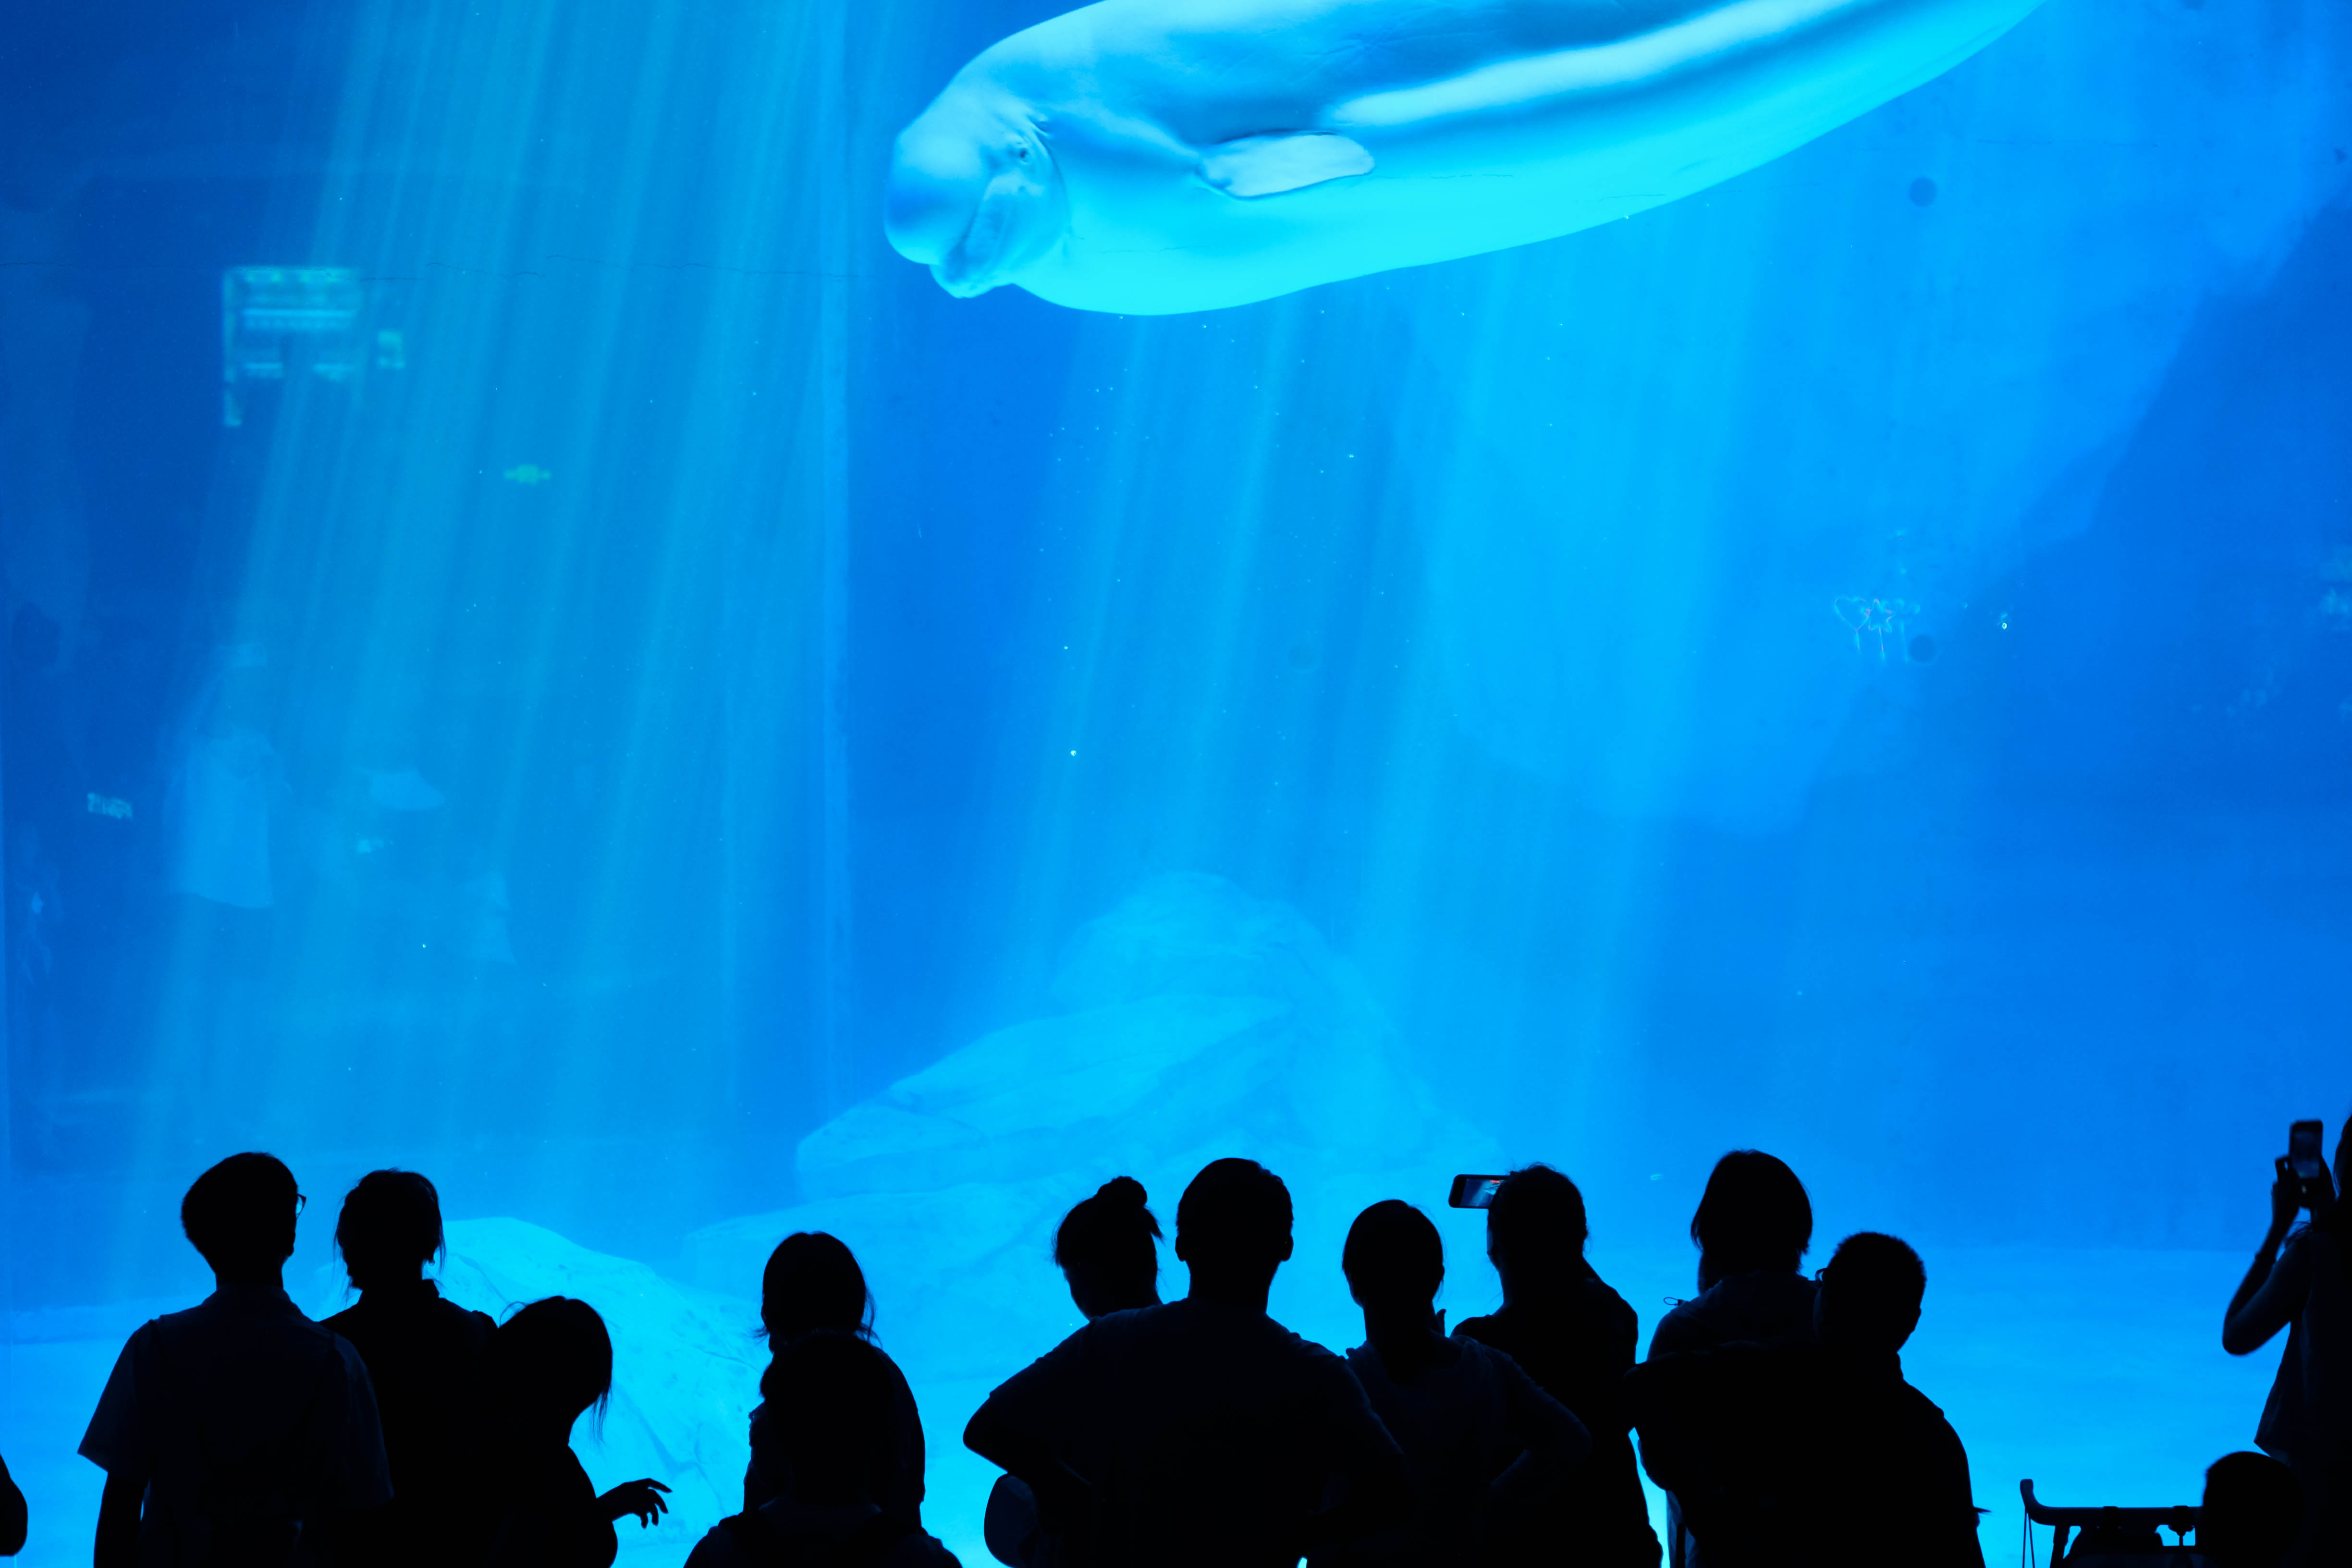
\includegraphics[width=\textwidth]{DSCF4489.jpg}
        \caption{\small T=0.28:0.3时，最后一秒内压力的偏差和}
        \label{fig:图4}
\end{minipage}
\end{figure}




\par
可以看出当T=0.288ms，50S后压力偏差和近似为0，即此时达到稳态。\par
综上可以得出结论，当单向阀每次开启的时长T=0.288ms时，高压油管内的压强尽稳定在100MPa左右，且偏差最小







\subsubsection{第二小问模型的建立与求解}

进一步分析，猜想不同开阀时长对应不同的稳态压力值，即当T确定时，从不同的初始状态
出发都会到达同一个稳态，不过到达稳态的时间不同。下面我们利用第一小问的模型，绘制了T=0.288ms时，
初始压强分别为100MPa和130MPa的压强变化图。
\begin{figure}[htbp]
    \centering
	\begin{minipage}{0.48\textwidth}
	    \centering
		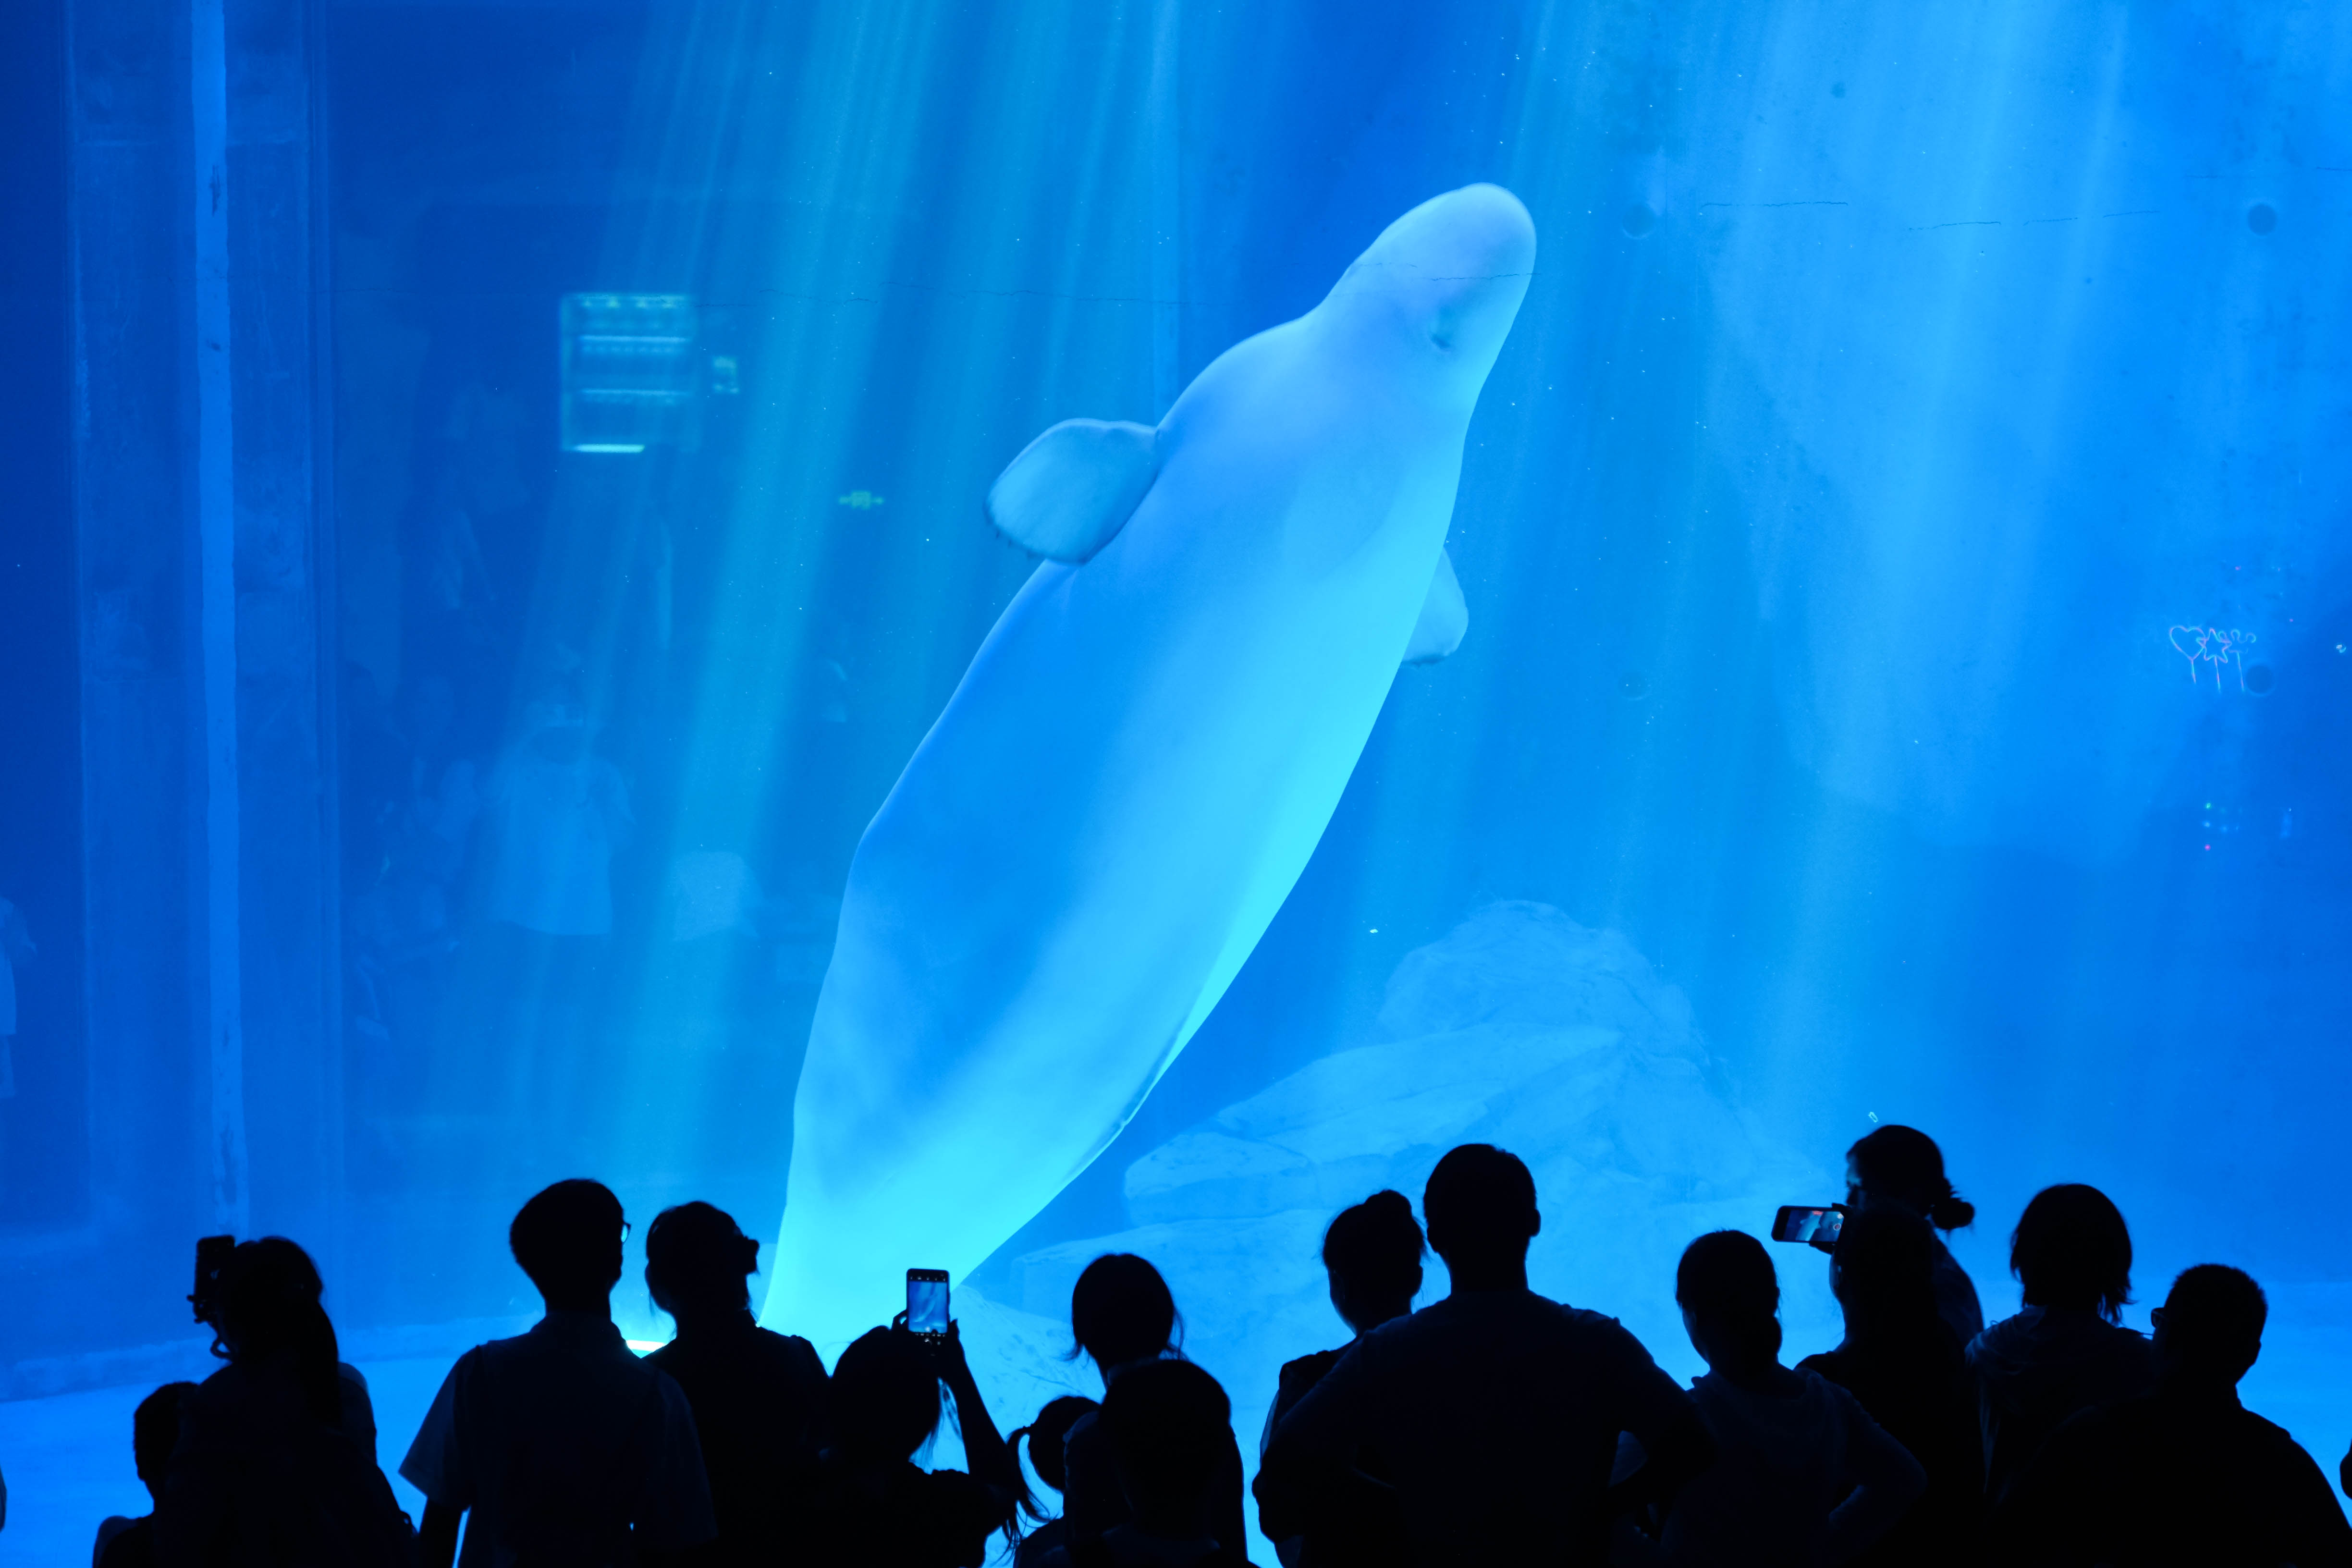
\includegraphics[width=\textwidth]{DSCF4490.jpg}
        \caption{\small 初始压力为100MPa，T=0.288ms}
        \label{fig:图5}

\end{minipage}
	\hfill
\begin{minipage}{0.48\textwidth}
\centering

		\includegraphics[width=\textwidth]{DSCF4501.jpg}
        \caption{\small 初始压力为130MPa，T=0.288ms}
        \label{fig:图6}
\end{minipage}
\end{figure}
\par
由图示以及计算稳态时的压强的均值，发现两个过程最后都在100MPa附近波动，证明猜想正确\par
另外，易知到达稳态所用的时间与T有关，T越大，到达稳态越迅速。\par
这表明了不同T的取值将对应唯一的系统稳态的压力均值$h_p(t)$；喷油开始时刻$t_0$和
初始压力的取值，对最终系统状态无影响。
\par
由模型稳态的描述，稳定时150MPa的期望压强应当对应唯一的单向阀开启时间。所以，可以先将
模型的期望压力设定为150MPa，得到对应单向阀开启时长$T_{150}$。然后研究该时长下系统达到150MPa的稳定压强
所需的时间。最后对2S，5S，10S的要求设计不同的调整方案。\par
在前一小问的基础上，将期望压强设定为$P_e=150MPa$，初始状态不改变；期望时间为$t_e$，喷嘴
开启时刻取$t_0=0$；利用前一小问的模型，得到对应$T_{150}$。利用一定时间内压强的均值$h_p(t)$
来描述整体压强，找到系统达到150MPa稳态所需要的时间$t_n$。分以下情况设计调整方案。
\\（1）若$t_e=t_n$
\par
系统刚好达到期望压强150MPa；
\\（2）若$t_e>t_n$
\par
在0到$t_n-t_e$时间内，单向阀开启时间不变化，$t_n-t_e$时刻调整为150MPa；
\\（3）若$t_e<t_n$
\par
此时$T_{150}$无法使得系统在规定的时间内达到150MPa的稳定压力。于是需要在0到$t_e$时间内使用更大的单向阀开启时长$T_m$使高压油管
升压到150MPa，然后再设定开启时长为$T_{150}$，使得系统状态稳定。\par
此时，对不同的$T_m$取值，令$t=t_e$，得到对应的$h_p(t)$，找到$h_p(t)$=150MPa即可。
\par
按照模型重复上述操作，可以得到$T_{150}=0.752ms$。对应实际压强变化如图：

\begin{figure}[htbp]
    \centering
	
	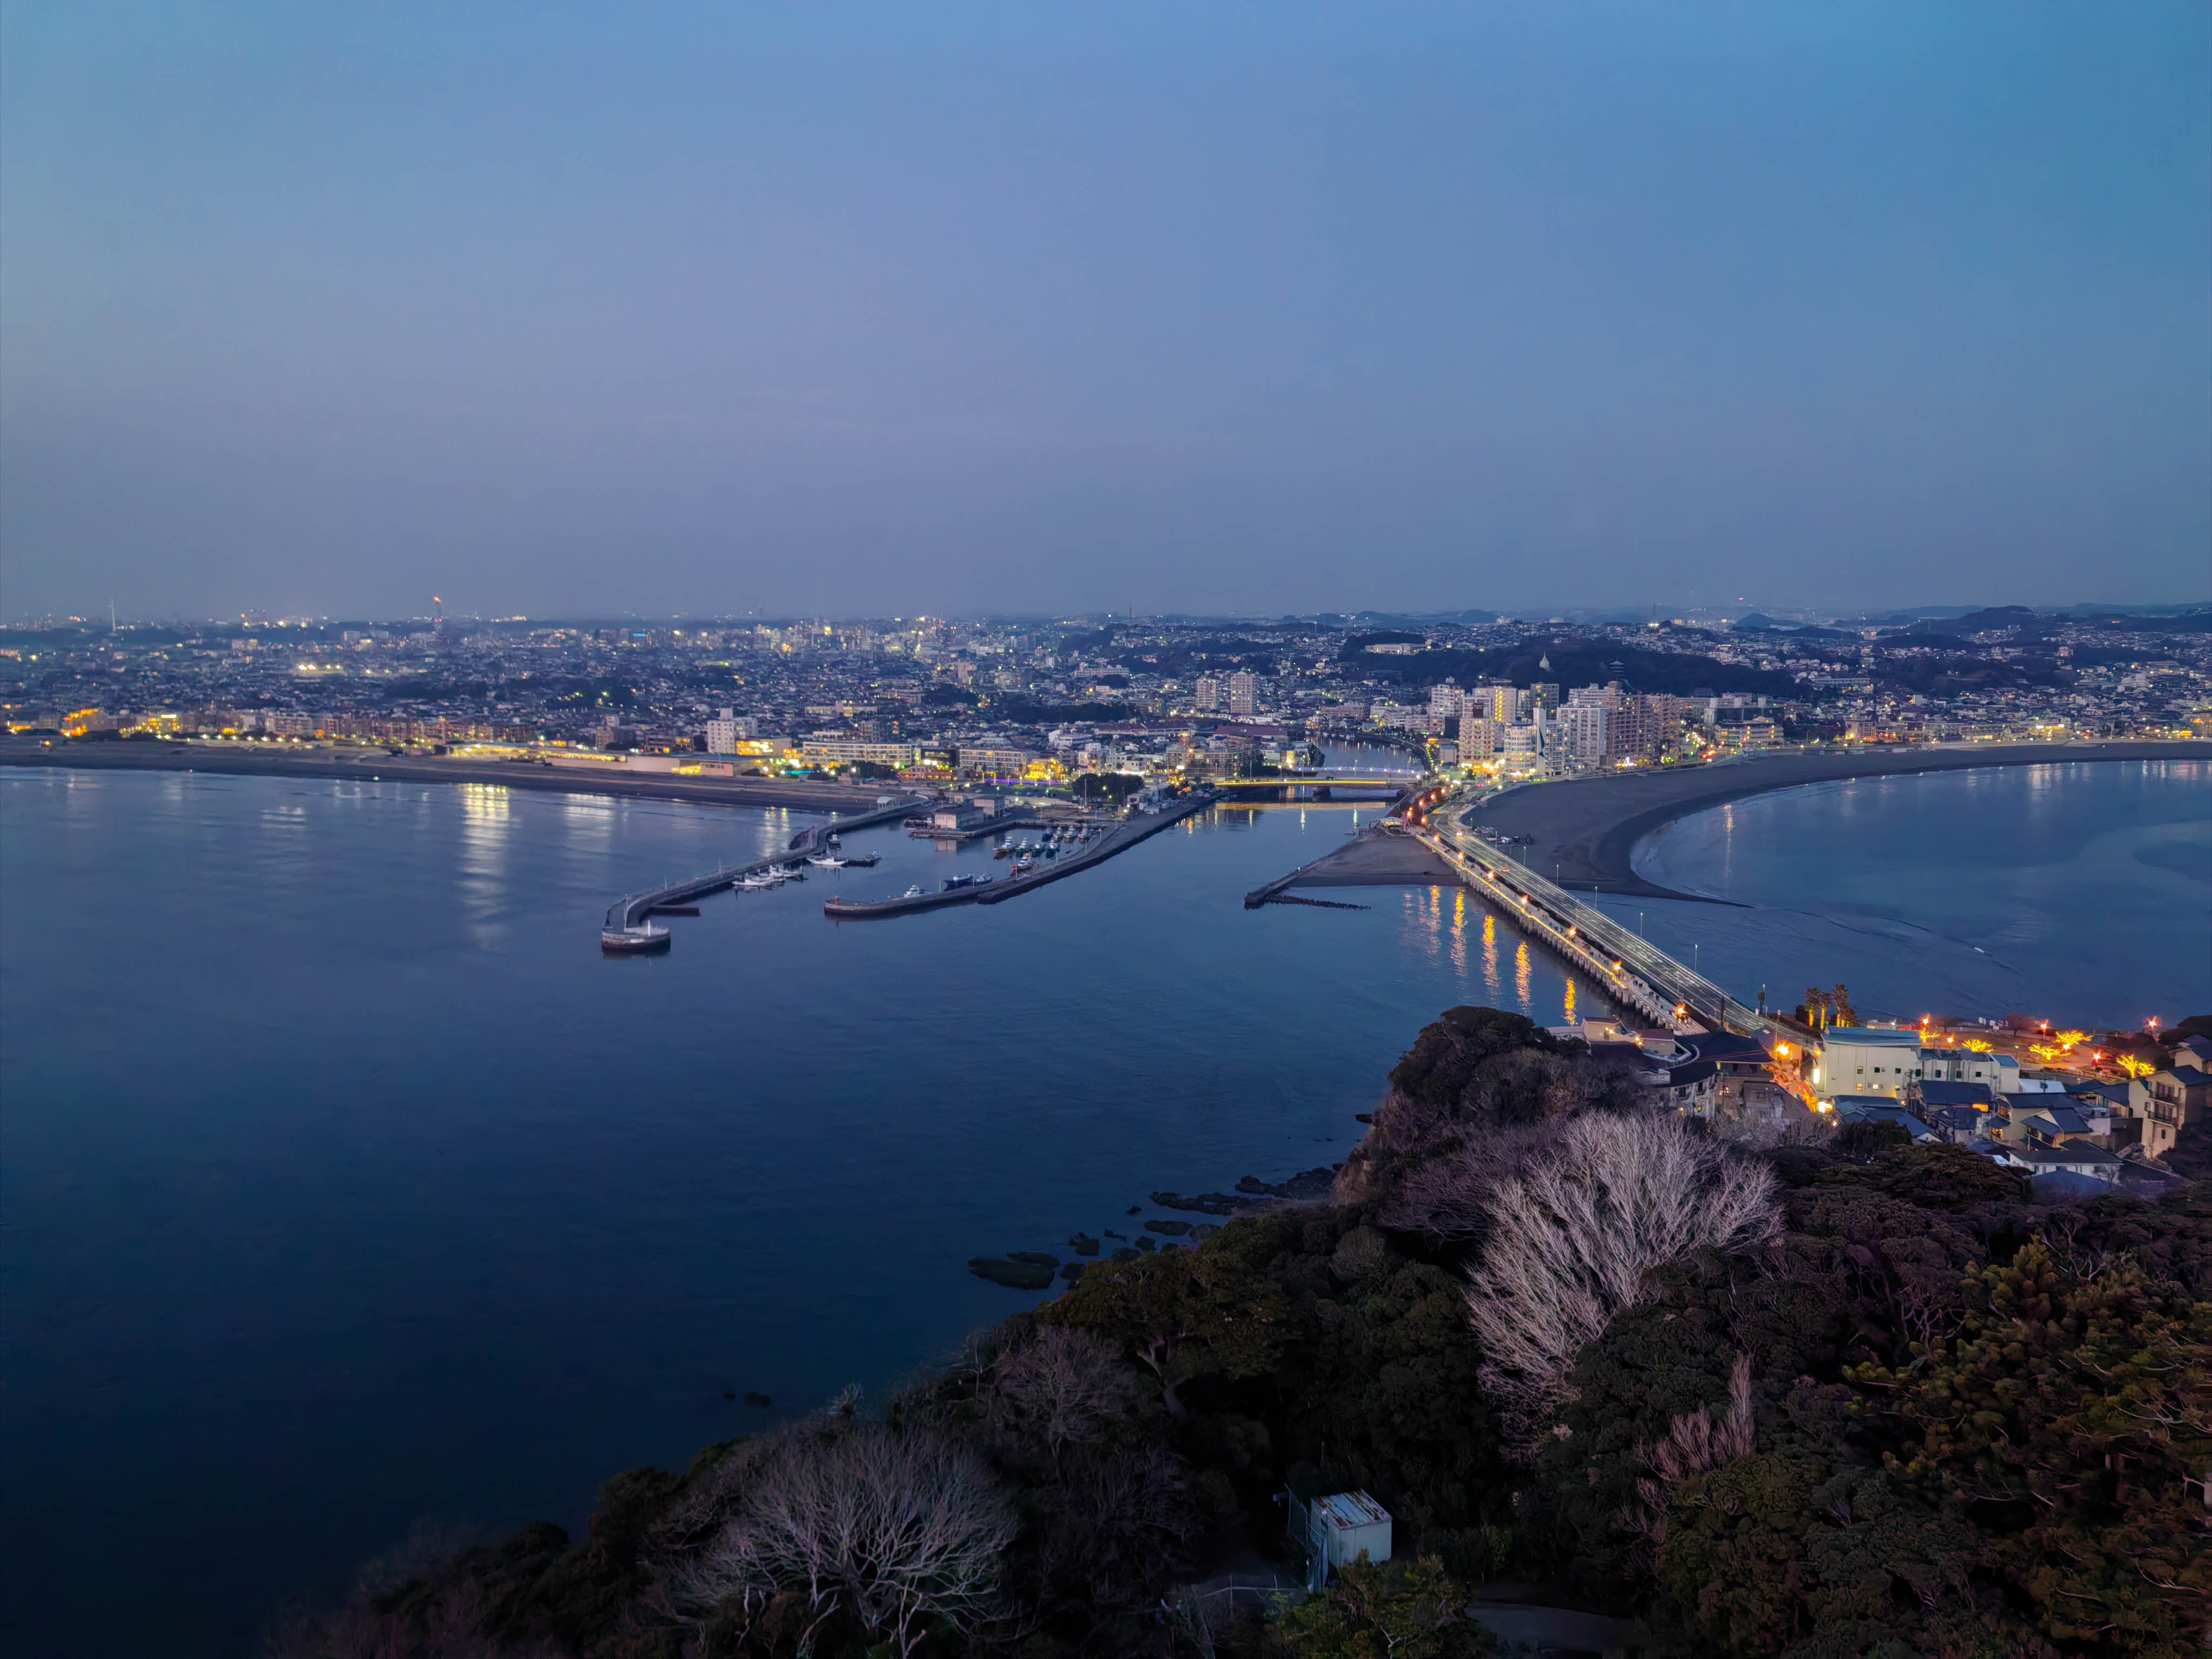
\includegraphics[width=0.8\textwidth]{enoshima-1.jpg}
    \caption{T=$T_{150}$时，系统实际压力随时间的变化}
    \label{fig:图7}


\end{figure}	

\par
令t取2000ms-6000ms，令一定时间内压强的均值$h_p(t)$取
\begin{equation} h_p(t)=\frac{\sum_{t-50}^{t+50} P(t)dt }{100}
\end{equation}
\\$h_p(t)$结果如图：

\begin{figure}[htbp]
    \centering
	
	\includegraphics[width=0.8\textwidth]{GBC贺图.jpg}
    \caption{T=$T_{150}$时，系统实际压力随时间的变化（局部放大）}
    \label{fig:图8}


\end{figure}	


\par
可以发现在5.9s时，系统达到150MPa的稳态，于是记$t_n=5900ms$\\
对于2s和5s，因为$t_e<5900ms$所以各自计算新的$t_n$。\\
（1）2s情况下\par
设$t_e=2000ms$，调整不同的单向阀开启时长$T_m$，得到不同的T值下2s时刻压强均值：

\par
可以得到$T_m=0.913ms$，方案为：0到2s取T=0.913ms，2S后取T=0.752ms

（2）5s情况下\par
设$t_e=5000ms$，调整不同的单向阀开启时长$T_m$，得到不同的T值下5s时刻压强均值：

	
\par
可以得到$T_m=0.755ms$，方案为：0到5s取T=0.755ms，2S后取T=0.752ms

（3）对于10s的要求：\par
由于$t_e=10000ms>t_n=5900ms$，于是方案为：在0-4.1s内保持T=0.288ms；4.1s时，调整T=0.755ms。
策略结果见下表。
\begin{table}[htbp]
	\centering
	\begin{tabular}{|c|c|}
		\hline
		{调整至稳定的时间} & {单向阀开启时长策略}\\ \hline
	    {2s} & {0到2s取T=0.913ms，2S后取T=0.752ms}\\ \hline
		{5s} & {0到5s取T=0.755ms，2S后取T=0.752ms}\\ \hline
		{10s} & {0-4.1s\text{内保持}T=0.288ms;4.1s\text{时，调整}T=0.755ms}\\ \hline
	\end{tabular}
	\caption{策略结果表}
	\label{tab:表1}
\end{table}

\subsection{问题三模型的建立与求解}
	%Part Six
	\section{模型的评价、改进与推广}
	\subsection{模型优点}
	\begin{enumerate}
		\item 
		\item 
		\item 
		\item 
	\end{enumerate}
	
	\subsection{模型缺点}
	\begin{enumerate}
		\item 
		\item 
		\item 
	\end{enumerate}
	
	\subsection{模型的改进}
	\begin{enumerate}
		\item 
		\item 
		\item 
	\end{enumerate}
	
	%Part Seven
	\section{参考文献}
	\vspace{-2em} % 减小上面的间距
	\begin{thebibliography}{9}  
		\bibitem{ref1} 
		\bibitem{ref2} 
		\bibitem{ref3} 
		\bibitem{ref4}   
	\end{thebibliography}
	
	\newpage
	\section*{附录}
	
	附录1：支撑材料的文件列表
 
	
	附录2：初始化代码和数据处理代码
	\begin{lstlisting}[language=python,columns=fullflexible,frame=shadowbox]
		import pandas as pd
		import warnings
		import xlwt
		import numpy as np
		import matplotlib.pyplot as plt
		import pylab
		import seaborn as sns
		from pylab import mpl
		from sklearn.preprocessing import PolynomialFeatures
		from sklearn import linear_model
		from sklearn.model_selection import train_test_split
		from sklearn.ensemble import RandomForestRegressor
		from sklearn import metrics
		import statsmodels.api as sm
		import geatpy as ea
		from scipy import  optimize as opt
		from scipy.optimize import minimize
	\end{lstlisting}
	
\end{document}